%-*- tex; tabsize:2; -*- %%%%%%%%%%%%%%%%%%%%%%%%%%%%%%%%%%%%%%%%%%%%%%%%%%%
%
%                          Copyright 2004-2005 JASSPA.
%                           All Rights Reserved
%
%
%  System        : MicroEmacs
%  Module        : user Manual
%  Object Name   : $RCSfile: jasspame.tex,v $
%  Revision      : $Revision: 1.6 $
%  Date          : $Date: 2005-03-12 21:16:54 $
%  Author        : $Author: jon $
%  Created By    : Jon Green
%  Created       : Mon Oct 25 21:36:13 2004
%  Last Modified : <050312.2111>
%
%  Description
%
%  Notes
%
%  History
%
%%%%%%%%%%%%%%%%%%%%%%%%%%%%%%%%%%%%%%%%%%%%%%%%%%%%%%%%%%%%%%%%%%%%%%%%%%%%%
%
% Copyright (c) 2004-2005 JASSPA.
%
% All Rights Reserved.
%
% This  document  may  not, in  whole  or in  part, be  copied,  photocopied,
% reproduced,  translated,  or  reduced to any  electronic  medium or machine
% readable form without prior written consent from JASSPA.
%
%%%%%%%%%%%%%%%%%%%%%%%%%%%%%%%%%%%%%%%%%%%%%%%%%%%%%%%%%%%%%%%%%%%%%%%%%%%%%

\documentclass[11pt,a4paper,pdftex]{article}
% Bring in the CVS information.
\def\CVS$#1: #2 ${\expandafter\def\csname CVS#1\endcsname{#2}}
\CVS$Revision: 1.6 $ % or any CVS keyword
\CVS$Date: 2005-03-12 21:16:54 $

\usepackage{ifthen}                     % Conditional processing.

\newboolean{Colorlinks}
\setboolean{Colorlinks}{true}              % For colored links

% Document information
%\newcommand{\docAuthor}{Jon Green, Kevin Garvey}
\newcommand{\docAuthor}{Jon Green}
\newcommand{\docSubject}{JASSPA MicroEmacs}
\newcommand{\docTitle}{Getting Started with JASSPA MicroEmacs}
\newcommand{\docDate}{\CVSDate}
\newcommand{\docVersion}{\CVSRevision}
\newcommand{\docReference}{jasspame}

% Import the font packages.
%\usepackage[latin1]{inputenc}  % We do not seem to need this
\usepackage{eurosym}            % Use the Euro symbol for "\euro"
\usepackage[T1]{fontenc}        % Refer to TeX psnfss2e.pdf
\usepackage{textcomp}           % Refer to TeX psnfss2e.pdf
\usepackage{aecompl}            % AE complement to T1 for "\NG" and "\ng"
\usepackage{color}              % Colored text boxes
\usepackage{calc}               % Allows calculations.
%
% FONTS: The document is typeset in the following fonts:-
% roman:      Times-Roman
% sans serif: Helvetica (scaled at .92)
% typewriter: Courier
\usepackage{courier}
\usepackage[scaled=0.92]{helvet}
%\usepackage{utopia}
\renewcommand{\rmdefault}{ptm}  % Roman font is Times-Roman
%\renewcommand{\rmdefault}{put}  % Utopia font is Times-Roman
\renewcommand{\sfdefault}{phv}  % Sans serif font is helvetica
\renewcommand{\ttdefault}{pcr}  % Typewriter font is courier

% Change the default font to Helvetica.
%\usepackage{bookman}
%\renewcommand{\familydefault}{\sfdefault}
%\renewcommand{\sfdefault}{ppl}

% Import the font packages.
\usepackage{pslatex}
\usepackage{longtable}                  % Long split table environment.
\usepackage{graphicx}                   % Picture import package
\usepackage{fancyhdr}                   % Use fancy headers
\usepackage[numbers]{natbib}            % Use Natural Sciences Citations and References

% Detect, if we are using pdftex to create pdf output. The following
% code should better be in a LaTeX package...
\makeatletter
\newif\ifpdfoutput
\@ifundefined{pdfoutput}%
  {\let\pdfoutput\@undefined}%
  {\ifcase\pdfoutput
     \let\pdfoutput\@undefined
   \else
     \pdfoutputtrue
   \fi
  }%
\makeatother

\usepackage{geometry,mflogo,xspace,path,bm}
\newcommand{\psext}{ps}
\newcommand{\pdfext}{pdf}
\newcommand{\dviext}{dvi}

% Set up the default link colour
\ifthenelse{\boolean{Colorlinks}}
{%
  \newcommand{\Linkcolor}{blue}
  \newcommand{\Citecolor}{red}
  \newcommand{\Urlcolor}{blue}
}
{%
  \newcommand{\Linkcolor}{black}
  \newcommand{\Citecolor}{black}
  \newcommand{\Urlcolor}{black}
}

\ifpdfoutput
  \pdfcompresslevel9
  \usepackage[colorlinks,bookmarks]{hyperref}
  \hypersetup{
    pdfauthor={\docAuthor},
    pdftitle={\docTitle},
    pdfsubject={\docSubject},
    pdfcreator={SunOS 5.9(sparc) - e-TeX(Web2C 7.5.2)},
    pdfkeywords={Emacs,MicroEmacs,Me,JASSPA},
    linkcolor={\Linkcolor},
    citecolor={\Citecolor},
    urlcolor={\Urlcolor},
    bookmarksnumbered=true,
    bookmarksopen=true
  }
  \usepackage{thumbpdf}
  \let\docext=\pdfext
\else
  \let\docext=\dviext
  \usepackage[bookmarks]{hyperref}
\fi

\title{\docTitle}
\author{Jon Green}
\date{\docDate}
%
% Bottom of the pages are ragged.
\raggedbottom
%
% Change the page width
%
\setlength{\marginparsep}{0pt}
\setlength{\marginparwidth}{0pt}
\addtolength{\textwidth}{.75in}
\addtolength{\hoffset}{-.25in}

\pagestyle{fancy}
% Set up the page.
% There is 1 inch at the top, reduce this to 0.4 inch.
\addtolength{\voffset}{-.6in}
\addtolength{\textheight}{.6in}
% We are adding a 1/2 inch graphic adjust the page sizes.
\setlength{\headheight}{.5in}
% Push page length to the bottom.
\addtolength{\textheight}{.5in}

%% Save the header image in a box
\newsavebox\HeaderImage
\savebox\HeaderImage{
\includegraphics[keepaspectratio,height=0.5in]{logo}}
% Redefine the header and footer for an alternative style.
\renewcommand{\sectionmark}[1]{\markright{\thesection\ #1}}
\fancyhf{}          % Delete the current header and footer
\fancyhead[EL,OR]{\bfseries\docTitle \\ \bfseries\rightmark}
\fancyhead[LO,RE]{\usebox{\HeaderImage}}
\fancyfoot[OL,ER]{{\small{Copyright {\textcopyright} 2004-2005 JASSPA.}}\linebreak
                   \textit{\small{\docReference~~v\docVersion~~\docDate}}}
\fancyfoot[EL,OR]{\textsf{\large \textbf{\thepage}}}
\renewcommand{\headrulewidth}{1.5pt}%
\renewcommand{\footrulewidth}{1.5pt}%

% Redefine a plain header and footer than is absent for the
% front page.
\fancypagestyle{plain}{%
  % Watermark for the first header. First we clear down the
  % existing header that may be defined.
  \fancyhead{}%
  % Refer to the "Using Imported Graphics in LaTeX2"
  % Define the header to appear on the left hand edge of the page.
  % The picture dimensions are specified as (0,0), this means that
  % it occupies zero space (as far as the layout engine is concerned).
  % Appearing in the header means that they are rendered before the
  % page itself.
  % The image is placed 0 inches to the left and -10inches below
  % the header. The graphics are then included such that the
  % aspect ratio is maintained and the image width is as wide as
  % the text width.
  \fancyhead[OL,ER]{\setlength{\unitlength}{1in}
%             \begin{picture}(0,0)
%               \put(0,-10){\includegraphics[keepaspectratio,width=\textwidth]{watermark}}
%             \end{picture}
  }
  \renewcommand{\headrulewidth}{0pt}  % Remove line
  \fancyfoot[EL,OR]{}
}

\newcommand{\tableTitle}[1]{\textbf{#1}}%   % used on all table titles.

\begin{document}
\pagenumbering{roman}           %%% Roman page numbers for ToC

%%%%%%%%%%%%%%%%%%%%%%%%%%%%%%%%%%%%%%%%%%%%%%%%%%%%%%%%%%%%%%%%%%%%%%%%%%%%%%
% New commands
\definecolor{CodeColor}{rgb}{0.95,0.95,0.95}
\newcommand{\CodeInsert}[1]{%
\vspace{3pt}
\colorbox{CodeColor}{\parbox{\textwidth}{\texttt{#1}}}
\vspace{3pt}
}
\newcommand{\CodeInsertW}[2]{%
\vspace{3pt}
\colorbox{CodeColor}{\parbox{#1}{\texttt{#2}}}
\vspace{3pt}
}

%%%%%%%%%%%%%%%%%%%%%%%%%%%%%%%%%%%%%%%%%%%%%%%%%%%%%%%%%%%%%%%%%%%%%%%%%%%%%%
%  Title Page                                                                %
%%%%%%%%%%%%%%%%%%%%%%%%%%%%%%%%%%%%%%%%%%%%%%%%%%%%%%%%%%%%%%%%%%%%%%%%%%%%%%
\thispagestyle{plain}
% The top header is the document information and the company logo. This is
% made up of 2 parbox's to get the correct horizontal wrapping that is
% required.
\parbox{2in}{
\includegraphics[keepaspectratio,width=1.9in]{logo}}
\hfill
\parbox{3.25in}{\sloppy
                \hfill\textsf{\huge JASSPA}
                \begin{flushright}
                  \textsf{\textbf{\Huge \docTitle}}
                \end{flushright}
                \hfill\textsf{\huge Version \docVersion}

                \hfill\textsf{\docAuthor}}
% The text information at the bottom of the page containing a copyright notice
% and contact details. This placed in a table and then shunted to the bottom
% of the page.
\begin{table}[b]
  \begin{center}
    \begin{tabular}{p{3in}p{3in}}
      \textsf{JASSPA}\vspace{6pt} & \\
      \textsf{\href{http://www.jasspa.com}{www.jasspa.com}\newline
              \href{mailto:support@jasspa.com}{support@jasspa.com}} & \\
%      \textsf{\sloppy\textbf{Copyright Notification:} No part of this
%      publication may be reproduced except as authorised by written
%      permission. The copyright and the foregoing restriction extend to
%      reproduction in all media.}
    \end{tabular}
  \end{center}
\end{table}

%%%%%%%%%%%%%%%%%%%%%%%%%%%%%%%%%%%%%%%%%%%%%%%%%%%%%%%%%%%%%%%%%%%%%%%%%%%%%%
%  Revision History                                                          %
%%%%%%%%%%%%%%%%%%%%%%%%%%%%%%%%%%%%%%%%%%%%%%%%%%%%%%%%%%%%%%%%%%%%%%%%%%%%%%
\newpage
% Change the format of the document to European paragraph spacing.
\setlength{\parindent}{0pt}
%\setlength{\parskip}{1ex plus 0.5ex minus 0.2ex}
\setlength{\parskip}{0.5ex}
\pagestyle{fancy}

\begin{small}
\vspace{.5in}
JASSPA.
\href{http://www.jasspa.com}{www.jasspa.com}\newline
\href{mailto:support@jasspa.com}{support@jasspa.com}\newline

\vspace{0.5in}

\textit{Copyright \textcopyright\ 2004-2005 JASSPA.}

% \textit{Copyright}

\vspace{0.5in}

\begin{table}[ht]
  \begin{tabular}{ll}
    Title:        & \docTitle \\
    Reference:    & \docReference \\
    Version       & v\docVersion \\
    Date:         & \docDate \\
  \end{tabular}
\end{table}

Typeset with the TexLive 2004 \LaTeX\ Documentation System under Sun Solaris 9.

\vspace{0.5in}

\begin{center}
  \begin{table}[ht]
    \begin{tabular}{|c|c|p{4in}|c|}
    \hline
    \tableTitle{Date} & \tableTitle{Who} & \tableTitle{Description} & \tableTitle{Revision} \\
    \hline
    2004/10/25 & Jon & Draft. & 1.00 \\ \hline
    \end{tabular}
  \end{table}
\end{center}
\end{small}

%%%%%%%%%%%%%%%%%%%%%%%%%%%%%%%%%%%%%%%%%%%%%%%%%%%%%%%%%%%%%%%%%%%%%%%%%%%%%%
% Introduction                                                               %
%%%%%%%%%%%%%%%%%%%%%%%%%%%%%%%%%%%%%%%%%%%%%%%%%%%%%%%%%%%%%%%%%%%%%%%%%%%%%%
\newpage
% Change the format of the document to European paragraph spacing.
\setlength{\parindent}{0pt}
%\setlength{\parskip}{1ex plus 0.5ex minus 0.2ex}
\setlength{\parskip}{0.5ex}
\pagestyle{fancy}

%\textbf{\Large Preface}
\pdfbookmark[1]{Preface}{intro}    %%% additional bookmark for ref
\markboth{Preface}{Preface}   %%% for the page header
\section*{Preface}
%\addcontentsline{toc}{section}{\numberline{}Preface}

Time is short, armed with a reasonable \LaTeX\ boiler plate it is time to put
down some usable notes on getting up and running with JASSPA MicroEmacs. The
on-line help that comes with JASSPA MicroEmacs details every public function
and variable in the editor however it is not that accessible and certainly
does not help the new user.

In this first draft, that will undoubtedly grow over time, we simply present
the post installation configuration to help the new user get up and running
with the editor.

Jon Green\newline
25th October 2004.

%%%%%%%%%%%%%%%%%%%%%%%%%%%%%%%%%%%%%%%%%%%%%%%%%%%%%%%%%%%%%%%%%%%%%%%%%%%%%%
% Table of Contents                                                          %
%%%%%%%%%%%%%%%%%%%%%%%%%%%%%%%%%%%%%%%%%%%%%%%%%%%%%%%%%%%%%%%%%%%%%%%%%%%%%%

\newpage
\pdfbookmark[1]{Contents}{toc}          %%% additional bookmark for ToC
\markboth{Table of Contents}{Table of Contents} %%% for the page header
\tableofcontents
\newpage

%%%%%%%%%%%%%%%%%%%%%%%%%%%%%%%%%%%%%%%%%%%%%%%%%%%%%%%%%%%%%%%%%%%%%%%%%%%%%%
% References                                                                 %
%%%%%%%%%%%%%%%%%%%%%%%%%%%%%%%%%%%%%%%%%%%%%%%%%%%%%%%%%%%%%%%%%%%%%%%%%%%%%%

\cleardoublepage
% Page numbering - continue the page numering from the arabic space. When we
% change to arabic space then the counter value is reset. Create a temporary
% counter to hold the page value from the `Roman' page space so that we
% commence the page numbering in `Arabic' space from where we left it. This
% technique ensures that the PDF page numbering is identical to that specified
% in the document.
\newcounter{pagetemp}                   % Temporary counter.
\setcounter{pagetemp}{\value{page}}     % Snoop the Roman page numbers
\pagenumbering{arabic}                  % From now on Arabic page numbers
\setcounter{page}{\value{pagetemp}}     % Align with Roman

% Change the format of the document to European paragraph spacing.
\setlength{\parindent}{0pt}
%\setlength{\parskip}{1ex plus 0.5ex minus 0.2ex}
\setlength{\parskip}{0.5ex}

\section{Installation and Setup}

\subsection{Installation}

To install JASSPA MicroEmacs then download the appropriate bundle from
\href{http://www.jasspa.com}{www.jasspa.com}. Most of the common platforms
include packages to simplify installation.

\subsubsection{Packaged Sun Solaris}

  As root install the package.

\CodeInsert{%
cd /tmp\newline
unzip jasspa-mepkg-sun-sparc-59-\textit{yyyymmdd}.zip\newline
pkgadd -d jasspa-me}

  The package is installed in \texttt{/opt/jasspa}. Edit your local login
  script file to include the executable on your local path e.g.
  \texttt{.cshrc} or \texttt{.profile} -- the syntax depends on the shell type
  that you use.

\CodeInsert{%
\#\newline
\# Set up Microemacs\newline
\#\newline
if [ -d /opt/jasspa ] ; then\newline
\hspace*{2em}PATH=\$PATH:/opt/jasspa/bin\newline
\hspace*{2em}MANPATH=\$MANPATH:/opt/jasspa/man\newline
fi\newline
...\newline
export PATH}

  The package may be subsequently removed using:

\CodeInsert{pkgrm jasspa-me}

\subsubsection{Packaged Red Hat Linux/Fedore Core}

  As root install the package.

\CodeInsert{rpm -i jasspa-me-\textit{yyyymmdd}-1.i386.rpm}

  The package is installed in directory \texttt{/usr/share/jasspa}, the
  executable is installed in \texttt{/usr/bin} and requires no additional
  setup.

  The package may be subsequently removed using:

\CodeInsert{rpm -e jasspa-me}

\subsubsection{Packaged HP-UX}

  For HP-UX then the package may be installed via SAM, but is easier to
  install using the command line:

\CodeInsert{/usr/sbin/swinstall -s `pwd`/jasspa-mepkg-hpux-pa-10.20-\textit{yyyymmdd}.depot jasspa-me}

  The package is installed in \texttt{/opt/jasspa}. The executable is
  automatically added to the shell profile environment. The user should log
  out and log back in again to pick up the new environment settings which are
  added to \texttt{/etc/profile}.

  The package may be subsequently removed using:

\CodeInsert{swremove jasspa-me}

\subsubsection{Packaged Microsoft Windows}

  Microsoft Windows environments 95/98/NT/2K/XP use an \textit{Install Shield}
  package installation which may be used to add and remove the package. The
  software is installed into \texttt{c:$\backslash$Program
  Files\-$\backslash$JASSPA\-$\backslash$MicroEmacs}.

  Unpack the \textit{zip} file, run \textbf{setup.exe} and follow the
  installation procedure.

\subsubsection{Non-packaged UNIX/Linux/BSD - System wide}

  For other UNIX/BSD environments where no package is provided then a manual
  installation is performed. Select the installation directory i.e.
  \texttt{/usr/local}.

\CodeInsert{cd /usr/local\newline
gunzip -c /\textit{path-to}/jasspa-metree-\textit{yyyymmdd}.tar.gz | tar xvf -}

    or using GNU tar

\CodeInsert{cd /usr/local\newline
gtar zxvf /\textit{path-to}/jasspa-metree-\textit{yyyymmdd}.tar.gz}

  The directory \texttt{/usr/local/jasspa} should now exist. Unpack the binary
  into the \texttt{/usr/local/bin} directory and make it executable.

\CodeInsert{cd /usr/local/bin\newline
gunzip -c /\textit{path-to}/jasspa-me-linux-2.\textit{x}-\textit{yyyymmdd}.gz > me\newline
chmod a rx me}

  The installation is complete, \texttt{/usr/local/bin} is assumed to be on 
  the executable path.

\subsubsection{Non-packaged UNIX/Linux/BSD - User Installation}

  For other UNIX/BSD environments where a local user install is required (i.e.
  the user has no permissions to write to the system directories) then the
  following steps may be followed.

  Unpack \textit{metree} in your home directory, this creates a directory tree
  called \textbf{jasspa}, once unpacked then rename the directory to
  \textbf{.jasspa}.

\CodeInsert{cd $\sim$\newline
gunzip -c /\textit{path-to}/jasspa-metree-\textit{yyyymmdd}.tar.gz | tar xvf -\newline
mv jasspa .jasspa}

  Add downloaded spelling dictionaries by unpacking them into the
  \texttt{$\sim$/.jasspa/spell} subdirectory. Install the binary into your local
  binary directory - we assume \texttt{$\sim$/bin} e.g.

\CodeInsert{cd $\sim$/bin\newline
gunzip -c /\textit{path-to}/jasspa-me-linux-2.\textit{x}-\textit{yyyymmdd}.gz > me\newline
chmod a+rx me}

  Assuming that the binary directory is already on the users path then the
  installation is complete.

\subsubsection{MS-DOS}

  For MS-DOS then no installation script is provided and a manual installation
  is performed. Select the installation directory, we shall assume
  \texttt{c:$\backslash$jasspa}.

  Unpack the \texttt{metree} zip package to form the macro tree, this creates
  the directory \textit{jasspa}.

\CodeInsert{c:\newline
cd $\backslash$\newline
unzip jasspa-metree-\textit{yyyymmdd}.zip}

  The binary is placed in the \texttt{c:$\backslash$jasspa} directory. It is
  important that the binary is placed in the JASSPA tree as this allows the
  executable to locate the \textit{macros} and \textit{spelling} directories
  without any further configuration. If the binary is placed in a separate
  location from the tree then the \textit{\$MExxxPATH} environment variables
  must be defined to enable the editor to locate the tree.

  Two different binaries are provided which are built with DJGPP V1.0 and
  V2.0. If you have DJGPP V2.0 installed in your system then install the V2.0
  binary, otherwise install the V1.0 binary (as this is a self contained
  executable and has no run-time library dependencies).

\CodeInsert{cd $\backslash$jasspa\newline
unzip jasspa-me-msdos-djgpp1-\textit{yyyymmdd}.zip}

  The location of the executable should be added to the \texttt{autoexec.bat}
  file e.g.

\CodeInsert{SET PATH=\%PATH\%;c:$\backslash$jasspa}

  The system may be re-booted and the editor should be available on the
  command line \texttt{me}.

\subsubsection{Windows Manual Installation}

  Manual installation is required under \textbf{Win32s} and may be optionally
  performed in \textbf{Win32} environments (95/98/NT/2K/XP). This is very
  similar to the \textbf{MS-DOS} installation.

  Unpack the \texttt{metree} zip package to form the macro tree, this creates
  the directory \textit{jasspa}. This is typically extracted to
  \textit{c:$\backslash$Program Files} (\textbf{Win32s} may use
  \textit{c:$\backslash$me}).

\CodeInsert{c:\newline
cd "$\backslash$Program Files"\newline
unzip jasspa-metree-\textit{yyyymmdd}.zip}

  The executable is placed in the \textit{jasspa} directory:

\CodeInsert{cd "$\backslash$Program Files$\backslash$jasspa"\newline
unzip jasspa-me-win32-\textit{yyyymmdd}.zip
}

  Unlike \textbf{MS-DOS} then short cuts are typically used to launch the
  editor. The editor short-cut is typically edited with command line option
  \textbf{-c} to restore the previous session when launched.

\subsubsection{Spelling Dictionaries}

  The spelling dictionaries are downloaded separately and are not included in
  the base packages, multiple dictionaries may be downloaded and installed for
  each language to be supported. Some languages include a \textit{base} and
  \textit{extended} dictionary, the \textit{base} contains the most popular
  words, the \textit{extended} includes more obscure words over and above the
  \textit{base}. The \textit{base} and \textit{extended} dictionary are
  packaged together, but the \textit{extended} dictionary may be removed when
  downloaded to conserve disk space.

  The spelling archive contains both the dictonaries and language specific
  macros required to install the dictionary into the system. All of the
  dictionaries are derrived from \textit{ispell} dictionaries. The Copyrights
  for each of the dictionaries are contained in the macro files.

  To install then the archive is unpacked into the \textit{jasspa/spelling}
  directory that was created when \textit{metree} was unpacked. Simply unpack
  the contents of the archive into this directory.

\CodeInsert{cd /\textit{path-to}/jasspa/spelling\newline
unzip enus.zip}

  With the directory installed then set up MicroEmacs using \textbf{Help
  $\rightarrow$ User Setup} or from the command line \textbf{M-x user-setup}.

  \begin{itemize}
    \item Select the \textbf{Platform} tab.

    \item Select the \textbf{Language} from the drop-down box.

    \item Enable \textbf{Auto Save Dictionaries} to automatically save the
    dictionary when new words are added or ignored.

    \item Enable \textbf{Enable Auto-Spell} if the auto spell facility is
    required. Auto-Spell performs background spell checking and highlights
    erroneous words.

  \end{itemize}

\subsection{Building from Source}

  Where a particular platform does not exist then MicroEmacs may be built from
  source. It is expected that the environment is set up with the appropriate
  tools to perform the build.

  A simple build script is provided for both UNIX and DOS/Windows systems
  called \textbf{build}. Download the source bundle
  \texttt{jasspa-mesrc-\textit{yyyymmdd}} and unpack, this will create a
  directory \textbf{meYYMMDD}. Change directory to \textbf{src} and issue a
  build command:

\CodeInsert{\# DOS\newline
c:> build}

\CodeInsert{\# UNIX\newline
>sh> ./build}

  On most systems then the \textbf{build} will be performed, alternatively an
  explicit \textbf{make} operation may be performed. A selection of
  \textit{make} files exist for different platforms \textbf{.mak}
  indicates a native platform compiler and \textbf{.gmk} indicates a GNU
  compiler.

\CodeInsert{make -f \textit{platform}.mak}

  The platform specific makefiles may be modified with compiler specific
  options for the target platform to produce a more optimal executable.

  For Microsoft Windows environments then a Microsoft Project file is
  provided.

\subsection{Running For the First Time}

  On running MicroEmacs for the first time with the command \textbf{me} then
  the user is asked to set up the environment. This process collects some very
  basic information and creates the user private files that store context and
  state. The user may decline to perform the set-up and is prompted next time
  the editor is executed.

  The environment is analyzed and the system directory locations and search
  paths are determined. These can typically be accepted as is.

  \begin{itemize}

    \item \textbf{Enter you full name ?} This is \textit{your} name that is
    inserted in the header files that identify you as the author.

    \item \textbf{Set up the company file (y/n) ?} If you are working in a
    company environment then this allows you to enter the name of the company
    that is used in copyright statements automatically inserted into new
    headers etc.

    \item \textbf{Name the company file ?} This is the name of the macro file
    that stores company wide company information. The default is simply called
    \textbf{company} and is typically accepted. If you are using a site wide
    installation then your system administrator may set up a specifically
    named company file which should be entered here.

    \item \textbf{Company Name ?} the long name of the company i.e.
    \textit{Acme Building Inc.}

  \end{itemize}

  The configuration is complete and the top level help page is displayed. The
  user should now perform the \textbf{User Setup} step detailed in a later
  section.

\subsection{Help Information}

  The help information is available on-line and may be accessed using the
  mouse or the keyboard.

\subsubsection{Mouse Interaction}

  \textbf{Help$\rightarrow$General Help}

  The links are shown highlighted and may be traversed with the mouse by
  selecting the link with a double click of the left button.

\subsubsection{Keyboard Interaction}

  \textbf{esc-x help}

  The links may be traversed using the \texttt{TAB} key to move to the next
  link, a \texttt{RETURN} on the link causes the link to be followed.

\subsection{User Setup}

  On completion of the basic configuration then a certain amount of
  customization is typically required. The \textit{User Setup} dialog allows
  the user to perform this process and is invoked as follows:

  \textbf{esc-x user-setup} $\dots$ \textit{OR}\newline
  \textbf{Help$\rightarrow$User Setup}

\begin{figure}[!hbt]
  \begin{center}
    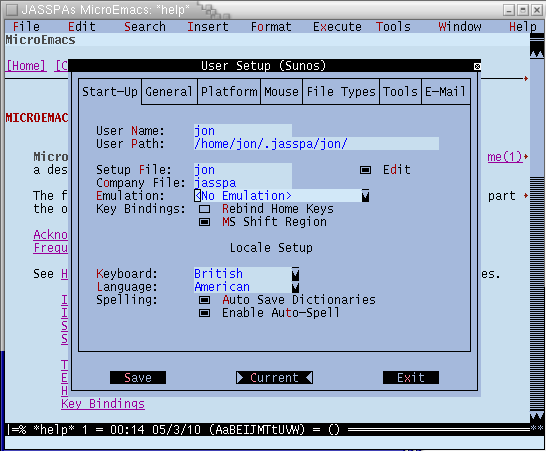
\includegraphics[keepaspectratio,height=3in]{usersetup}
    \caption{User Setup Dialog}
    \label{fig:usersetup}
  \end{center}
\end{figure}

  Navigation within the dialog is performed using the mouse and/or
  \texttt{TAB} and cursor keys. The \texttt{SPACE} key is used to open a drop
  down dialog. The configuration may be saved permanently using \textbf{Save}
  and installed into the current session using \textbf{Current}.

\subsubsection{Common Options}

  For a quick setup then the \textit{User Setup} dialog is traversed by tab,
  the most common options are described below, other options may be ignored. 
  In a console environment use the cursor keys to move from tab to tab whilst 
  the tab is in focus.

  \begin{itemize}
    \item \textbf{Start-up} -- start up configuration information.

    \begin{itemize}

      \item \textbf{Emulation} select the preferred emulation mode of the
      editor. The standard key bindings are adjusted to be more consistent
      with the selected emulation. if the emulation is changed then it is
      advisable to re-start the editor when \textit{User Setup} is complete. 

      \item \textbf{Re-bind Home Keys} when disabled then the keys
      \textit{Home} and \textit{End} move to the beginning and end of the
      buffer respectively. When enabled then \textit{Home} and \textit{End}
      move to the beginning and end of the line respectively.

      \item \textbf{MS Shift Bindings} enabled performs Microsoft region
      selection using the cursor keys whilst the \texttt{SHIFT} key is
      pressed.

      \item \textbf{Keyboard} select your keyboard type, the keyboard bindings
      are corrected for the locale.

      \item \textbf{Language} the default spelling language. This has no
      effect if the dictionaries are not loaded.

      \item \textbf{Auto Save Dictionaries} typically enabled, causes the user
      defined spelling dictionary to be automatically saved on exiting the
      editor.

      \item \textbf{Enable Auto-spell} enable this option to allow MicroEmacs
      to perform spell checking whilst you type. Spelling errors are
      highlighted to indicate errors. With the mouse right click on the
      mis-spelt word and select an auto correction.

      \textbf{M-x auto-spell-buffer} to automatically spell check the
      whole buffer.

      \textbf{M-x spell-buffer} to spell check the buffer via spell dialog.

    \end{itemize}

    \item \textbf{General} -- general defaults and settings.

    \begin{itemize}

      \item \textbf{Full Name} user name that is inserted into new file
      templates.

      \item \textbf{Main Menu} disable if the Main Menu is not required.

      \item \textbf{Alt Action} defines the behavior of the \texttt{ALT} key.
      Enable \textbf{Esc Prfx} if the \texttt{ALT} key may be used as a
      \texttt{ESC} key prefix (most Emacs users). Disable \textbf{Main menu
      Hot-keys} if the \texttt{ALT} key should not be used as a hot key to the
      Main menu. When both are enabled then the Main menu has priority.

      \item \textbf{Abbrev Setup} defines the behavior of the abbreviation key
      binding \textbf{esc esc}.

      \begin{itemize}

        \item Enabling \textbf{Accent} completes accented characters i.e.
        \texttt{:o<esc><esc>} is converted to a \texttt{\"{o}}.

        \item Enabling \textbf{Lookback} attempts to complete the word based
        on previous words in the buffer. A further \textbf{esc esc} finds the
        previous etc.

        \item Enabling \textbf{Dict'n} attempts to complete a word based on
        the spelling dictionary.

      \end{itemize}

      \item \textbf{Tab to Indent} controls the behavior of the TAB key. By
      default, where indent rules exist for a buffer then the \texttt{TAB} key
      causes the indentation of the line to be re-evaluated rather than
      inserting a literal \texttt{TAB} character. Select the operation
      required, the default is \textit{Always Indent}.

    \end{itemize}

    \item \textbf{Platform} -- general platform specific settings.

    \begin{itemize}

      \item \textbf{Termcap Color (Termcap Only)} enables use of colors.

      \item \textbf{Use Fonts (Termcap Only)} enables use of \textbf{bold} and
      \underline{underline} fonts.

      \item \textbf{Font Name} selection of an alternative fixed font. For
      UNIX then use \textbf{xfontsel} to select a font to paste into the
      window. For MS-Windows then use the \textbf{Choose Font} button to
      select the font.

      \item \textbf{Enable Tool Bar} enable if the tool bar at the left of the
      screen is required. Add tools to the tool bar, this provides short cuts,
      itemized lists for specific buffers. The tool bar is buffer sensitive.

      \item \textbf{Ignore files} the list of files to be ignored in directory
      listings. e.g. \texttt{~ .o CVS}

      \item \textbf{Fence Display} defines the behavior of the cursor at fence
      characters (i.e. \texttt{(,\{,\},),..}). \textbf{Always draw and jump on
      close} is the most popular, the brackets are colorized and the cursor
      jumps to the opening fence on entering a close. A miss-matched fence is
      highlighted in an error color.

      \item \textbf{Scroll Bars} generally \textbf{Wide with Splitter} is
      preferred in desktop environments. A wide scroll bar is two characters 
      wide, the \textit{splitter} is a control point to split the window with 
      the mouse.

      \item \textbf{Horizontal Scroll} defines the behavior of horizontal
      scrolling when the cursor is moved to the end of the line. By default
      only the current line is scrolled.

      \item \textbf{Vertical Scroll} defines the behavior of vertical
      scrolling when the cursor is moved down at the top/bottom line of the
      window. For terminals then \textbf{Default, half screen} is preferred,
      for graphical environments then \textbf{Smooth, Single line} is
      preferred.

      \item \textbf{Color Scheme} the highlighting color of the buffer window.
      In a console environment then use the special scheme for
      \textit{Termcap}.

    \end{itemize}

    \item \textbf{Mouse} -- behavior of the mouse.

    \begin{itemize}

      \item \textbf{Mouse Button Bindings} control the action on pressing a
      button, optionally in conjunction with the \texttt{SHIFT},
      \texttt{CONTROL} and \texttt{ALT} modifier keys. The wheel mouse setting
      is bound here.

    \end{itemize}

  \end{itemize}

\subsection{MicroEmacs Integration}

  This section discusses how MicroEmacs may be integrated with the desktop
  environment and other tools.

\subsubsection{Desktop Integration}

  Integration of MicroEmacs with the Window Manager desktop environment.

  \begin{itemize}

    \item Drag and Drop is supported. When a file(s) is dragged over a buffer
    window and released then the file(s) is opened in the drop window.

    \textbf{UNIX} environments support \textit{Xdnd}. Under X-Windows the
    MicroEmacs window is not raised following the drop.

    \textbf{Microsoft Windows} the MicroEmacs window is raised following
    a drop operation.

    \item Different size bitmaps are provided for the desktop.

    \textbf{UNIX} icons are provided in
    \texttt{\textit{/path-to}/jasspa/pixmaps} in both \textbf{png} and
    \textbf{pixmap} format. A set of additional file type MicroEmacs icons may
    be downloaded for use with Gnome, KDE and CDE.

    \textbf{Microsoft Windows} different size bitmaps are provided in the icon
    executable file \textbf{meicons.exe}. This executable contains the
    standard JASSPA icon in addition to the file type icons. Select icons from
    this executable when assigning MicroEmacs to specific file extensions.

    \item When assigning MicroEmacs to a desktop icon then it is advisable to
    start MicroEmacs with the command line option \textbf{-c}. This option
    restores the editor to the previously loaded state of the last saved
    session.

    \item Where MicroEmacs is assigned as an open action for a given file type
    or extension then an existing editor session may be used rather than
    opening a new editor. To enable MicroEmacs to reuse an existing session
    then invoke \textbf{me} with the \textbf{-o} command line option and
    enable the \textbf{Client-Server} configuration option (\textbf{Help
    $\rightarrow$ User Setup $\rightarrow$ Platform $\rightarrow$ Client
    Server}).

    \item The size and the position of the MicroEmacs frame position may be
    defined at startup. There are a number of different methods to set the
    frame characteristics as follows:-

    \begin{itemize}

      \item \textbf{Frame Size} the simplest method to fix the frame size at
      start up is to resize the frame to the desired size. Once resized, with
      the mouse \textit{Right Click} on the \textit{mode line} and select
      \textbf{Store Frame Size}. The current frame size is saved and restored
      the next time the editor is started.

      \item \textbf{UNIX -- Size and Position} may be controlled using the
      \textbf{.Xdefaults} file, an entry in the file

      \CodeInsertW{\textwidth-\leftmargin}{MicroEmacs.geometry: 102x65 60 30}

      defines the frame size to be 102 characters wide, 65 characters deep and
      should be positioned 60 pixels from the left screen edge and 30 pixels
      from the top screen edge.

      \item \textbf{Windows -- Size and Position} may be controlled using the
      \textbf{me32.ini} file, an entry in the file

      %5.75in
      \CodeInsertW{\textwidth-\leftmargin}{[Defaults]\newline
      \textit{; Define startup screen size.}\newline
      geometry=102x65+60+30}

      defines the frame size to be 102 characters wide, 65 characters deep and
      should be positioned 60 pixels from the left screen edge and 30 pixels
      from the top screen edge. This entry is in \textbf{[Defaults]} and
      therefore applies to all users, for a single user configuration then use
      the section labeled \textbf{[\textit{logname}]} where \textit{logname}
      is the users Windows login name.

    \end{itemize}

  \end{itemize}

\subsubsection{Application Integration}

  MicroEmacs may be invoked from other tools as the selected text editor (i.e.
  \textbf{WinZip}). Multiple files may be specified on the command line for
  opening. Where a specific line number is required then the command line
  option \textbf{-l \textit{lineNo}} may be used to open the next file and
  move to the given line number. The \textbf{-l} must always precede the file
  name, but may appear multiple times in the command line before  each file
  to be open. e.g.

  \CodeInsert{me -l 20 foo.c -l 902 bar.c}

  which opens file \texttt{foo.c} displaying line 20 and opens \texttt{bar.c}
  displaying line 902.

\subsubsection{Utilities Integration}

  MicroEmacs optionally uses the standard UNIX utilities such as
  \textbf{grep}, \textbf{find} and \textbf{diff} for searching for information
  from the file system when present. These tools are typically found as
  default on a UNIX system.

  Where the tools are \underline{not} on the execution path, or the tool
  default options are altered, then the tools should be declared to MicroEmacs
  in your \textbf{\textit{username}.emf} file. Table~\ref{tab:com} defines
  the variables which are associated with the utility execution.

  \begin{table}[ht]
   \begin{center}
    \begin{tabular}{lll}
    \textbf{Variable} & \textbf{Description} \\ \hline
    \textbf{\%man-com} & \texttt{man} utility, find and display reference pages.\\
    \textbf{\%find-com} & \texttt{find} utility, find files.\\
    \textbf{\%grep-com} & \texttt{grep} utility, search a file for a pattern.\\
    \textbf{\%diff-com} & \texttt{diff} utility, compare two files.\\
    \textbf{\%gdiff-com} & \texttt{diff} utility, graphical compare of two files.\\
    \textbf{\%cvs-com} & \texttt{cvs} utility, Concurrent versions system.\\
    \textbf{\%compile-com} & \texttt{make} utility, build command line. \\ \hline
    \end{tabular}
    \caption{External Command Variables}
    \label{tab:com}
   \end{center}
  \end{table}

  The command defaults are platform specific, but are typically defined as
  follows:

  \CodeInsert{%
  set-variable \%man-com "man"\newline
  set-variable \%find-com "find"\newline
  set-variable \%grep-com "grep -n"\newline
  set-variable \%diff-com "diff -r -c"\newline
  set-variable \%gdiff-com "diff -w"\newline
  set-variable \%find-com "find"\newline
  set-variable \%cvs-com "cvs"\newline
  set-variable \%compile-com "make"}

\subsubsection{Microsoft Windows UNIX utilities}

  Microsoft Windows does not include the standard UNIX utilities by default,
  they may be downloaded from
  \href{http://unxutils.sourceforge.net/}{http://unxutils.sourceforge.net/}.
  Alternatively \textbf{cygwin} binaries may be used if installed.

  The tools should be declared to MicroEmacs in your
  \textbf{\textit{username}.emf} file, typically located in directory
  \textbf{c:$\backslash$Documents and
  Settings$\backslash$\textit{username}$\backslash$Application
  Data$\backslash$jasspa}.

  With the \textbf{unxutils} standard installation
  then the tools are defined in \textbf{\textit{username}.emf} as follows:

  \CodeInsert{set-variable \%grep-com "c:/unix/usr/local/wbin/grep.exe -n"\newline
  set-variable \%find-com "c:/unix/usr/local/wbin/find.exe"\newline
  set-variable \%diff-com "c:/unix/usr/local/wbin/diff.exe -c -d -b -r"\newline
  set-variable \%gdiff-com "c:/unix/usr/local/wbin/diff.exe -c -w"}

  The directory path and options should be modified to match \textit{your}
  version of the tools.

\subsubsection{Microsoft Windows and Cygwin}

  MicroEmacs integrates with \textbf{Cygwin}
  (\href{http://www.cygwin.com}{www.cygwin.com}) allowing a \textbf{Bash}
  shell to be opened up in a window using the command \textbf{M-x\ cygwin}.
  Additionally the MicroEmacs commands \textbf{M-x man} and \textbf{M-x
  info} are available to access the Cygwin Manual and Info pages,
  respectively.

  If cygwin is installed in the default location \texttt{c:$\backslash$cygwin}
  then MicroEmacs automatically detects the directory and enables support. If
  cygwin has been installed in a different location then this should be
  defined to MicroEmacs in \textbf{\textit{username}.emf} using the variable
  \texttt{\%cygwin-path} as follows, correcting for your installation location:

  \CodeInsert{set-variable \%cygwin-path "c:/cygwin"}

\cleardoublepage
\section{MicroEmacs Basics}

  In this chapter we introduce the basic information that you need to control
  MicroEmacs. MicroEmacs is equipped with a wealth of features and it is
  virtually impossible to describe each and every one in detail. For the new
  user then MicroEmacs is sometimes incorrectly perceived as difficult, there is
  a minimal set of commands which are required to drive the editor
  effectively, once mastered then you will find that MicroEmacs provides a fast and
  effective platform for handling text.

\subsection{Getting Started}

  To start MicroEmacs then simply type the command \textbf{me} (or
  \textbf{me32} on MS-Windows) followed by the filename(s) to edit e.g.

  \CodeInsert{me myfile}

  The editor should start and load the file \textit{myfile}. If the file does
  not exist no error is reported and the user is presented with an empty file,
  subsequently saving that buffer will create the file. If the file is a
  directory then a directory listing is presented.

  If MicroEmacs is started with the command option \textbf{-c} then the last
  editing session is restored i.e.

  \CodeInsert{me -c }
  
  additional files may be specified with \textbf{-c} if required.

\subsection{MicroEmacs Screen}

  On starting MicroEmacs then the screen layout is as depicted in
  Figure~\ref{fig:basicscreen}.

  \begin{figure}[!hbt]
    \begin{center}
      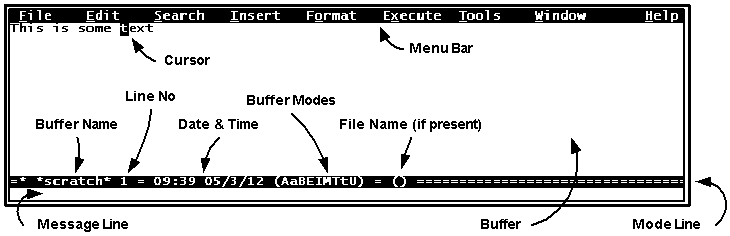
\includegraphics[keepaspectratio,width=5in]{basicscreenannot}
      \caption{Basic Screen Layout}
      \label{fig:basicscreen}
    \end{center}
  \end{figure}

  At the top of the screen is the \textbf{Menu Bar}, highlighted characters
  indicate the hot key that brings up the menu item using
  \texttt{ALT-\textit{key}}. The menu may be accessed with the mouse or hot
  keys. If the Main Menu association has been disabled in \textit{User Setup}
  then the \texttt{F1} key may be used to bring up the first menu item,
  thereafter the cursor and menu hot keys permit navigation.

  At the bottom of the screen is the \textbf{Mode Line} which provides
  information on the buffer that is being edited, including the \textit{buffer
  name}, \textit{file name}, \textit{line number} and abbreviated
  \textit{buffer modes}. Where several buffers are on screen at the same time
  then each buffer has its own Mode Line.

  The last line of the screen is the \textbf{Message Line} which is used to
  display messages and is used for command entry.

\subsection{Files, Buffers and Windows}

  When editing a \textit{file} then MicroEmacs copies that file into a
  \textit{buffer} held in memory, the buffer has a name which is typically the
  base name of the file. The buffer is presented to the user in a
  \textit{window}, the window typically has a scroll bar allowing the view
  into the buffer to be changed.

  Changes to the buffer modify the in memory copy only, the file contents are
  not changed until the buffer is saved when it overwrites the original file
  with the new contents. A backup file(s) may be created with the previous
  file contents allowing the user to restore the previous version if
  necessary. During an editing session then a periodic automatic save is
  performed every few minutes to a recovery file, should the system
  unexpectedly crash then MicroEmacs will recover the automatic save the next
  time the file is loaded.

  MicroEmacs allows multiple buffers to be loaded into the system at any time,
  not all buffers are necessarily visible, the user controls which buffers to
  display in a \textit{window}. The windows may be split horizontally or
  vertically allowing the same, or different, buffer to be viewed in another
  window i.e. you are allowed to have two (or more) window views into a
  buffer. Editing in one window immediately affects other windows that are
  viewing the same buffer.

  Buffers may be created independently of a file, these are typically named
  with a preceeding asterisk (\texttt{*}) character, i.e. \texttt{*scratch*}
  which always exists in the system and may be used for temporary working.

  Buffers may be saved to files, when a buffer is saved to a different file
  then a new file is created or existing file is over-written. As a side
  effect the buffer name is changed to reflect the new file name.

\subsection{Modes}

  MicroEmacs uses \textit{modes} to customize the behavior of commands, a set
  of global modes exist which are inherited by all buffers that are created.
  Buffers themselves may change the mode to alter local buffer behavior.

  The global modes are set up in \textit{User Setup}, buffer modes are
  modified in the local buffer using:

  \begin{itemize}
    {\setlength{\itemsep}{0ex}}
    \item \textbf{C-x~m} toggle buffer mode.
    \item Right mouse click in the buffer or on the mode line.
    \item \textbf{C-x buffer-setup} to permanently redefine the modes
    associated with the buffer.
  \end{itemize}

  The common buffer modes are defined as follows:

  \begin{longtable}{l@{\ --\ }p{5.8in}}
    \endhead
    \endfoot
    \endlastfoot

    \textbf{auto} & when enabled performs automatic source file line type
    detection (i.e. UNIX, DOS, Windows) \\

    \textbf{autosv} & when enabled performs periodic auto-save backup of
    changes.\\

    \textbf{exact} & when enabled makes searching and replace case sensitive.\\

    \textbf{fence} & when enabled performs automatic fence matching i.e.
    \texttt{(..)} pairs.\\

    \textbf{over} & when enabled overwrites rather than inserts entered
    characters, \textbf{insert} key.\\

    \textbf{indent} & when enabled a new line of text automatically inherits
    the previous lines left indent.\\

    \textbf{magic} & when enabled assumes a regular expression search and
    replace.\\

    \textbf{quiet} & when enabled disables audio beep on an error.\\

    \textbf{tab} & when enabled spaces are used instead of literal \texttt{TAB}
    characters.\\

    \textbf{time} & when enabled files are automatically time stamped with
    the edit time.\\

    \textbf{undo} & when enabled retains undo information.\\

    \textbf{view} & when enabled the buffer is read only and cannot be
    modified.\\

    \textbf{wrap} & when enabled automatic text wrapping is performed at the
    \textit{fill column}.\\

  \end{longtable}

\subsection{Keys and the Keyboard}

  MicroEmacs is keyboard biased, this is the fastest way to control the
  editor. Throughout this manual we discuss commands and the keys on the
  keyboard that invoke those commands. MicroEmacs uses a special key sequence
  nomenclature to describe the commands.

  \begin{description}

    \item[C-] the control key and another key pressed at the same time.
    \textbf{C-x} is the \texttt{CONTROL} and \texttt{X} key pressed at the
    same time, this sequence is a prefix key sequence that starts many
    MicroEmacs commands.

    \item[M-] this is a special key called META which is used to start many
    commands. The META key is typically \texttt{ESC} but may also be the
    \texttt{ALT} key pressed with another key. To enable the use of
    \texttt{ALT} then this should be enabled in \textit{User Setup}.
    \textbf{M-a} indicates the \texttt{ESC} key followed by the \texttt{A} key
    or \texttt{ALT} and \texttt{A}, this may also be written as \textbf{esc
    a}.

    \item[S-] the \texttt{SHIFT} key. \textbf{S-pagedown} is the
    \texttt{SHIFT} key and \texttt{PageDown} keys pressed at the same time.

    \item[insert] a special named key found on the keyboard i.e.
    \texttt{INSERT}, \texttt{RETURN}, \texttt{BACKSPACE}. The special key
    names are always lowercase.

  \end{description}

  A sequence of multiple keys is described with a minus sign
  (\textbf{\texttt{-}} to indicate that the keys are pressed together (a
  slight exception to this rule is \textbf{M-a} when \texttt{ESC} is used as
  \texttt{ESC} is pressed first followed by the \texttt{A} key). Where keys
  follow each other then a \textbf{SPACE} character is used. e.g.

  \begin{longtable}{l@{\ --\ }l}
    \endhead
    \endfoot
    \endlastfoot
    \textbf{C-x C-c} & \texttt{CONTROL}-\texttt{X} followed by
                       \texttt{CONTROL}-\texttt{C}.\\

    \textbf{C-z a} & \texttt{CONTROL}-\texttt{X} followed by \texttt{A}.\\
    \textbf{M-space} & \texttt{ALT} and \texttt{SPACE} or \texttt{ESC} followed
                       by \texttt{SPACE}.\\
    \textbf{S-f1} & \texttt{SHIFT} and \texttt{F1} function key.\\
  \end{longtable}

\subsection{Entering Text}

  Entering text in MicroEmacs is easy, simply type in text and \texttt{RETURN}
  to start a new line. MicroEmacs does not wrap text by default and will
  scroll the line to keep it within the window as more text is typed.
  MicroEmacs will automatically wrap the text if \textbf{wrap} mode is
  enabled.

  You can change the wrap mode setting using the following commands:

  \textbf{C-x m} wrap.\newline
  \textbf{Right Mouse} on mode line and select \textbf{Buffer Modes}.\newline
  \textbf{C-x buffer-mode}\newline
  \textbf{C-x buffer-setup}

  For most text buffer types then \textbf{wrap} mode is always enabled, for
  programming languages then it is typically disabled. Within a text type
  buffer then a paragraph is denoted by a empty line, paragraphs may be laid
  out using \textbf{M-o} \textit{fill-paragraph} which re-styles the
  paragraph.

\subsection{Cursor Movement}

  Navigation around the buffer is performed with cursor keys or with the
  following control sequences:

  \begin{longtable}{ll@{\ --\ }l}
    \endhead
    \endfoot
    \endlastfoot
    \textbf{C-f} & \textit{forward-char} &
    Forward character.\\
    \textbf{C-b} & \textit{backward-char} &
    Backward character.\\
    \textbf{C-n} & \textit{forward-line} &
    Next line.\\
    \textbf{C-p} & \textit{backward-line} &
    Previous line.\\
    \textbf{C-v}, \textbf{page-down} & \textit{scroll-down} &
    Next page.\\
    \textbf{C-z}, \textbf{page-up} & \textit{scroll-up} &
    Previous page.\\
  \end{longtable}

  To move to the extremities of the line or buffer:

  \begin{longtable}{ll@{\ --\ }l}
    \endhead
    \endfoot
    \endlastfoot
    \textbf{C-a} & \textit{beginning-of-line} &
    Goto start of line.\\
    \textbf{C-e} & \textit{end-of-line} &
    Goto end of line.\\
    \textbf{M-<}, \textbf{home} & \textit{beginning-of-buffer} &
    Goto start of buffer.\\
    \textbf{M->}, \textbf{end} & \textit{end-of-buffer} &
    Goto end of buffer.\\
  \end{longtable}

  To move between words and paragraphs then the keys are similar to the basic
  cursor movement but are modified by \texttt{META}.

  \begin{longtable}{ll@{\ --\ }l}
    \endhead
    \endfoot
    \endlastfoot
    \textbf{M-f}, \textbf{C-right} & \textit{forward-word} &
    Goto the next word.\\
    \textbf{M-b}, \textbf{C-left} & \textit{backward-word} &
    Goto the previous word.\\
    \textbf{M-n}, \textbf{M-]} & \textit{forward-paragraph} &
    Goto next paragraph.\\
    \textbf{M-p}, \textbf{M-[} & \textit{backward-paragraph} &
    Goto previous paragraph.\\
  \end{longtable}

  Finally, to move to a specific line:

  \begin{longtable}{ll@{\ --\ }l}
    \endhead
    \endfoot
    \endlastfoot
    \textbf{M-g} & \textit{goto-line} &
    Prompt for a line number and jump to it.\\
  \end{longtable}

\subsection{Abort and Exiting}

  The \underline{most} important command is \textbf{C-g} \textit{abort}. If
  you are in the middle of executing a command or are in a unrecognized state
  then \textbf{C-g} will abort the current command and restore the user to a
  sane state.

  To exit MicroEmacs:

  \begin{longtable}{ll@{\ --\ }l}
    \endhead
    \endfoot
    \endlastfoot
    \textbf{M-z} & \textit{quick-exit} &
    Saved unsaved buffers and exit.\\
    \textbf{C-x~C-c} & \textit{save-buffer-exit-emacs} &
    Prompts user to save unsaved buffers and exits.\\
  \end{longtable}

\subsection{Loading and Saving Files}

  When the editing is complete then the file may be saved using the command
  \textbf{C-x~C-s} \textit{save-buffer}. If there is no name associated with a
  buffer then no save is possible and the buffer should be written to a
  different file. To save a buffer to a different file then the command
  \textbf{C-x~C-w} \textit{write-buffer} is used. The user is prompted for the
  name of the file to save.

  To load a file into a new buffer then use the command \textbf{C-x~C-f}
  \textit{find-file}. Control is moved to the \textit{Message Line} for file
  entry. Within the Message Line then use the \texttt{TAB} key (or
  \textbf{esc~esc}) to auto-complete, a second \texttt{TAB} displays a list of
  possible completions. Enter the a few characters and use the \texttt{TAB} to
  complete again. Once the filename has completed then use \texttt{RETURN} to
  perform the read.

  Whilst in the Message Line performing a \textbf{C-x~C-f} then if
  \texttt{RETURN} is entered at a directory then a directory listing is
  displayed. The directory may be traversed by moving the cursor to the
  filename and pressing \texttt{RETURN} or by selecting a directory name with
  the mouse. If the selected item in the directory listing is a file then the
  file is loaded into a buffer.

  A summary of the buffer commands:

  \begin{longtable}{ll@{\ --\ }l}
    \endhead
    \endfoot
    \endlastfoot
    \textbf{C-x~C-f} & \textit{find-file} &
    Loads a file into a buffer.\\
    \textbf{C-x~C-s} & \textit{save-buffer} &
    Save buffer back to the file.\\
    \textbf{C-x~C-w} & \textit{write-buffer} &
    Save buffer to a new file.\\
    \textbf{C-x~C-i} & \textit{insert-file} &
    Insert a file at the current cursor position.\\
    \textbf{C-x~C-v} & \textit{view-file} &
    Loads a file into a buffer read-only (i.e. cannot be changed).\\
    \textbf{C-x~k} & \textit{kill-buffer} &
    Deletes the current buffer.\\
  \end{longtable}

\subsection{Insertion and Deletion}

  By default MicroEmacs operates in \textbf{insert} mode, the \textbf{insert}
  key toggles \textit{insertion} and \textit{overwrite}.

\subsubsection{Region Copy/Delete}

  Text may be deleted using the following keys:

  \begin{longtable}{ll@{\ --\ }l}
    \endhead
    \endfoot
    \endlastfoot
    \textbf{backspace} & \textit{backward-delete-char} &
    Delete the previous character behind the cursor.\\
    \textbf{delete} & \textit{forward-delete-char} &
    Delete the character under the cursor.\\
  \end{longtable}

  Sections of text may be copied (\textit{yanked}) or deleted after they have
  been marked up. MicroEmacs uses a \textit{Mark} position \textbf{C-space}
  \textit{set-mark} to define the start of the block and \textit{Point}, which
  is the current cursor position, to identify a \textit{region}.

  To mark up a region then use one of the following methods:-

  \begin{itemize}

    \item \textbf{Using the mouse}
    \begin{itemize}
      \item Use the mouse to place the cursor at the start of the region.
      \item Press the left key, keeping it pressed move the cursor to the end
      of the region.
    \end{itemize}

    \item \textbf{Using the keyboard}
    \begin{itemize}
      \item Use the cursor keys to move to the start of the region.
      \item Place a mark using \textbf{C-space} \textit{set-mark}.
      \item Use the cursor keys to move to the end of the region.
    \end{itemize}

    \item \textbf{Using the Keyboard -- Mircosoft Shift Region method} this is 
      only if Microsoft Shift region is enabled in \textit{User Setup}.
    \begin{itemize}
      \item Use the cursor keys to move to the start of the region.
      \item Hold down the shift key whilst moving the cursor keys, a region
      will be defined.
    \end{itemize}
  \end{itemize}

  Once the region is defined then the region may be copied to the \textit{yank
  buffer} or deleted:

  \begin{longtable}{ll@{\ --\ }l}
    \endhead
    \endfoot
    \endlastfoot
    \textbf{M-w} & \textit{copy-region} &
    Copy the selected region.\\
    \textbf{C-w} & \textit{kill-region} &
    Delete the selected region.\\
  \end{longtable}

\subsubsection{Yank (or paste)}

  A copied or deleted region may be inserted back into the text by moving the
  cursor to the insertion position and yanking (\textit{paste}) the text back
  using \textbf{C-y} \textit{yank}. \textbf{yank} is typically bound to the
  middle mouse button, inserting text under the mouse pointer position.

  The yank buffer has 20 entries, if a \textbf{M-y} \textit{reyank} operation
  is performed immediately after a \textit{yank} operation then the previous
  yank buffer contents are used. This allows previous text that has been
  copied or killed to be restored. The yank buffer remains valid when moving
  between different buffers, allowing text to be copied from one buffer to
  another.

  \begin{longtable}{ll@{\ --\ }l}
    \endhead
    \endfoot
    \endlastfoot
    \textbf{C-y} & \textit{yank} &
    Restore a copied or deleted text region.\\
    \textbf{M-w} & \textit{reyank} &
    Restore the previous copied or deleted text region.\\
  \end{longtable}

\subsubsection{Undo}

  MicroEmacs by default maintains an \textit{undo} history allowing recovery
  from editing mistakes. \textit{undo} is by default enabled and is changed by
  the \textbf{undo} mode. The undo information remains valid until a save
  operation is performed when it is discarded. The undo may be retained
  between saves by enabling the user option \textit{User Setup::General::Keep
  Undo}.

  \begin{longtable}{ll@{\ --\ }l}
    \endhead
    \endfoot
    \endlastfoot
    \textbf{C-\_} & \textit{undo} &
    Undo the last edit operation.\\
  \end{longtable}

\subsection{Buffers and Windows}

  Experienced users of MicroEmacs typically use more than one buffer
  (sometimes hundreds when running a long session) and continually move
  between different buffers. Typically only two or three \textit{windows} will
  be used (depending on screen estate), a working window and other window.

\subsubsection{Buffers}

  The buffer commands are:

  \begin{longtable}{ll@{\ --\ }l}
    \endhead
    \endfoot
    \endlastfoot
    \textbf{C-x~C-b} & \textit{list-buffers} &
    List the buffers in the system.\\
    \textbf{C-x~b} & \textit{find-buffer} &
    Find the named buffer (\texttt{TAB} to complete on the Message Line).\\
    \textbf{C-x~x} & \textit{next-buffer} &
    Move to the next buffer.\\
  \end{longtable}

  If you are not familier with the buffer commands then the simple way to
  change buffer is to use the mouse. Right click in the buffer window and
  select the \textbf{Buffer..} item and a list of current buffers is
  displayed. Left click to select the required buffer.

  On a console then the simple way to change the buffer is to use
  \textbf{C-x~C-b} \textit{list-buffers} change windows and move to the
  required buffer, enter \texttt{1} and the buffer is opened.

\subsubsection{Windows}

  The \textit{window} provides a view into a \textit{buffer}, MicroEmacs
  supports up to 64 windows on screen at once. The windows may be created from
  the keyboard or mouse. Refer to the notes in a later section on using the
  mouse in the windowing system.

  When buffers are swapped in and out of the windows then the buffer position
  is retained so that when the buffer is restored to the window then the
  cursor and line position are the same as when the buffer was previously in
  view.

  The essential window commands are:

  \begin{longtable}{ll@{\ --\ }l}
    \endhead
    \endfoot
    \endlastfoot
    \textbf{C-x~2} & \textit{split-window-vertically} &
    Split window into 2, \textit{stacked}.\\
    \textbf{C-x~3} & \textit{split-window-horizontally} &
    Split window into 2, \textit{side-by-side}.\\
    \textbf{C-x~1} & \textit{delete-other-windows} &
    Delete the other windows leaving current.\\
    \textbf{C-x~p} & \textit{previous-window} &
    Move to the previous window.\\
    \textbf{C-x~o} & \textit{next-window} &
    Move to the next window.\\
  \end{longtable}

\subsection{Searching and Replacing}

  Searching and replacement of text are frequently used in MicroEmacs, the
  search is probably the most important and runs using \textit{incrementally}.
  This is different from most other systems which require you to enter the
  whole search string. The incremental search starts searching from the first
  character that you type in allowing the search to be refined as it continues
  through the buffer.

\subsubsection{Searching}

  The search command is initiated using \textbf{C-s} \textit{isearch-forward},
  the user is placed on the Message Line. As characters are entered then the
  search proceeds through the buffer until a match is found and are displayed.
  if the user wishes to continue then refine the search by entering more
  characters or find the next match by entering another \textbf{C-s}. If the
  correct location in the file has been located then any other command will
  quit the search leaving the cursor at the current position (e.g.
  \textbf{C-f} or a cursor key). If the end of the buffer is reached then the
  user is warned, a further \textbf{C-s} will continue the search from the
  start of the buffer, effectively wrapping the buffer.

  A search in a backward direction is initiated with \textbf{C-r}
  \textit{isearch-backward} this operates in the same way as the forward
  search except the direction is changed.

  The search is sensitive to the buffer modes:

  \begin{description}
    \item[exact] when enabled performs a case sensitive search, the default is
      case insensitive.

    \item[magic] when enabled performs a regular expression search, in
    \textbf{magic} mode then some characters are reserved as follows:

      \begin{description}
        \item[.] Wildcard character.
        \item[$\wedge$] Start of the line.
        \item[$\backslash\backslash$] Backslash character, $\backslash$ is
        treated as an escape character and must be escaped for a literal
        backslash.
        \item[\$] End of the line.
        \item[{[}a-z{]}] Range of characters, use a caret ($\wedge$) at the
        start of range to negate the character set.
        \item[$\backslash$(\textit{pattern}$\backslash$|\textit{altpattern}$\backslash$)]
        \textit{pattern} group, optionally with \textit{alternative patterns}.
        \item[\textit{pattern}*] Zero or more occurrences of the previous \textit{pattern}.
        \item[\textit{pattern}+] One or more occurrences of the previous \textit{pattern}.
      \end{description}

  \end{description}

\subsubsection{Replacing}

  Replacing text is a powerful way to make global changes to a file and is
  invoked with \textbf{M-\%} or \textbf{M-C-r} \textit{query-replace-string}.
  This is an interactive replacement where the user controls the replacement,
  other replacement commands exist without the query.

  On invoking the command then the user is prompted for the search string
  followed by the replacement string. MicroEmacs then commences the search and
  prompts the user for the required action when the search pattern is found.
  The user responses are defined as follows:

  \begin{description}
    \item[?] provide help on the command response.
    \item[y] perform the replacement.
    \item[n] no skip the replacement and find the next.
    \item[!] perform the rest of the replacements with no query.
    \item[u] undo the last replacement.
    \item[C-g] abort the replacement and leave the cursor at the current
    position.
    \item[.] abort the replacement and leave the cursor at the point where the
    replace command was started.
  \end{description}

  As with the search, the replacement is affected by the buffer \textbf{exact}
  and \textbf{magic} modes. The regular expression search and replace allows
  patterns found in the search string to be copied to the replacement string,
  refer to the manual pages for more information.

\subsection{Named Command Executation}

  Not all of MicroEmacs commands are bound to keys, for example the named
  command that has no key binding is \textbf{user-setup}. To execute a named
  command then we use \textbf{M-x \textit{command}}
  \textit{execute-named-command}. MicroEmacs prompts the user for the
  \textit{command} to execute, at the prompt the \texttt{TAB} or
  \textbf{esc~esc} will attempt to complete the command, this is similar to
  the file name completion.

\subsection{Universal Repeat}

  All of MicroEmacs commands may be executed \textit{n} times using the
  \textbf{esc~n \textit{command}} \textit{universal-argument}. Entering
  \textbf{esc} followed by an integer \textit{n} executes the next command
  \textit{n}-times. e.g.

  \CodeInsert{\textbf{esc 12 C-n}}

  moves forward 12 lines (\textbf{C-n} is \textit{forward-line}).

  \CodeInsert{\textbf{esc 100 C-y}}

  inserts 100 copies of the yank buffer.

\subsection{Mouse Interaction}

  The mouse interaction shown in Figure~\ref{fig:basicmouse} depicts multiple
  buffer windows and a toolbar (leftmost Window).

  \begin{figure}[!h]
    \begin{center}
      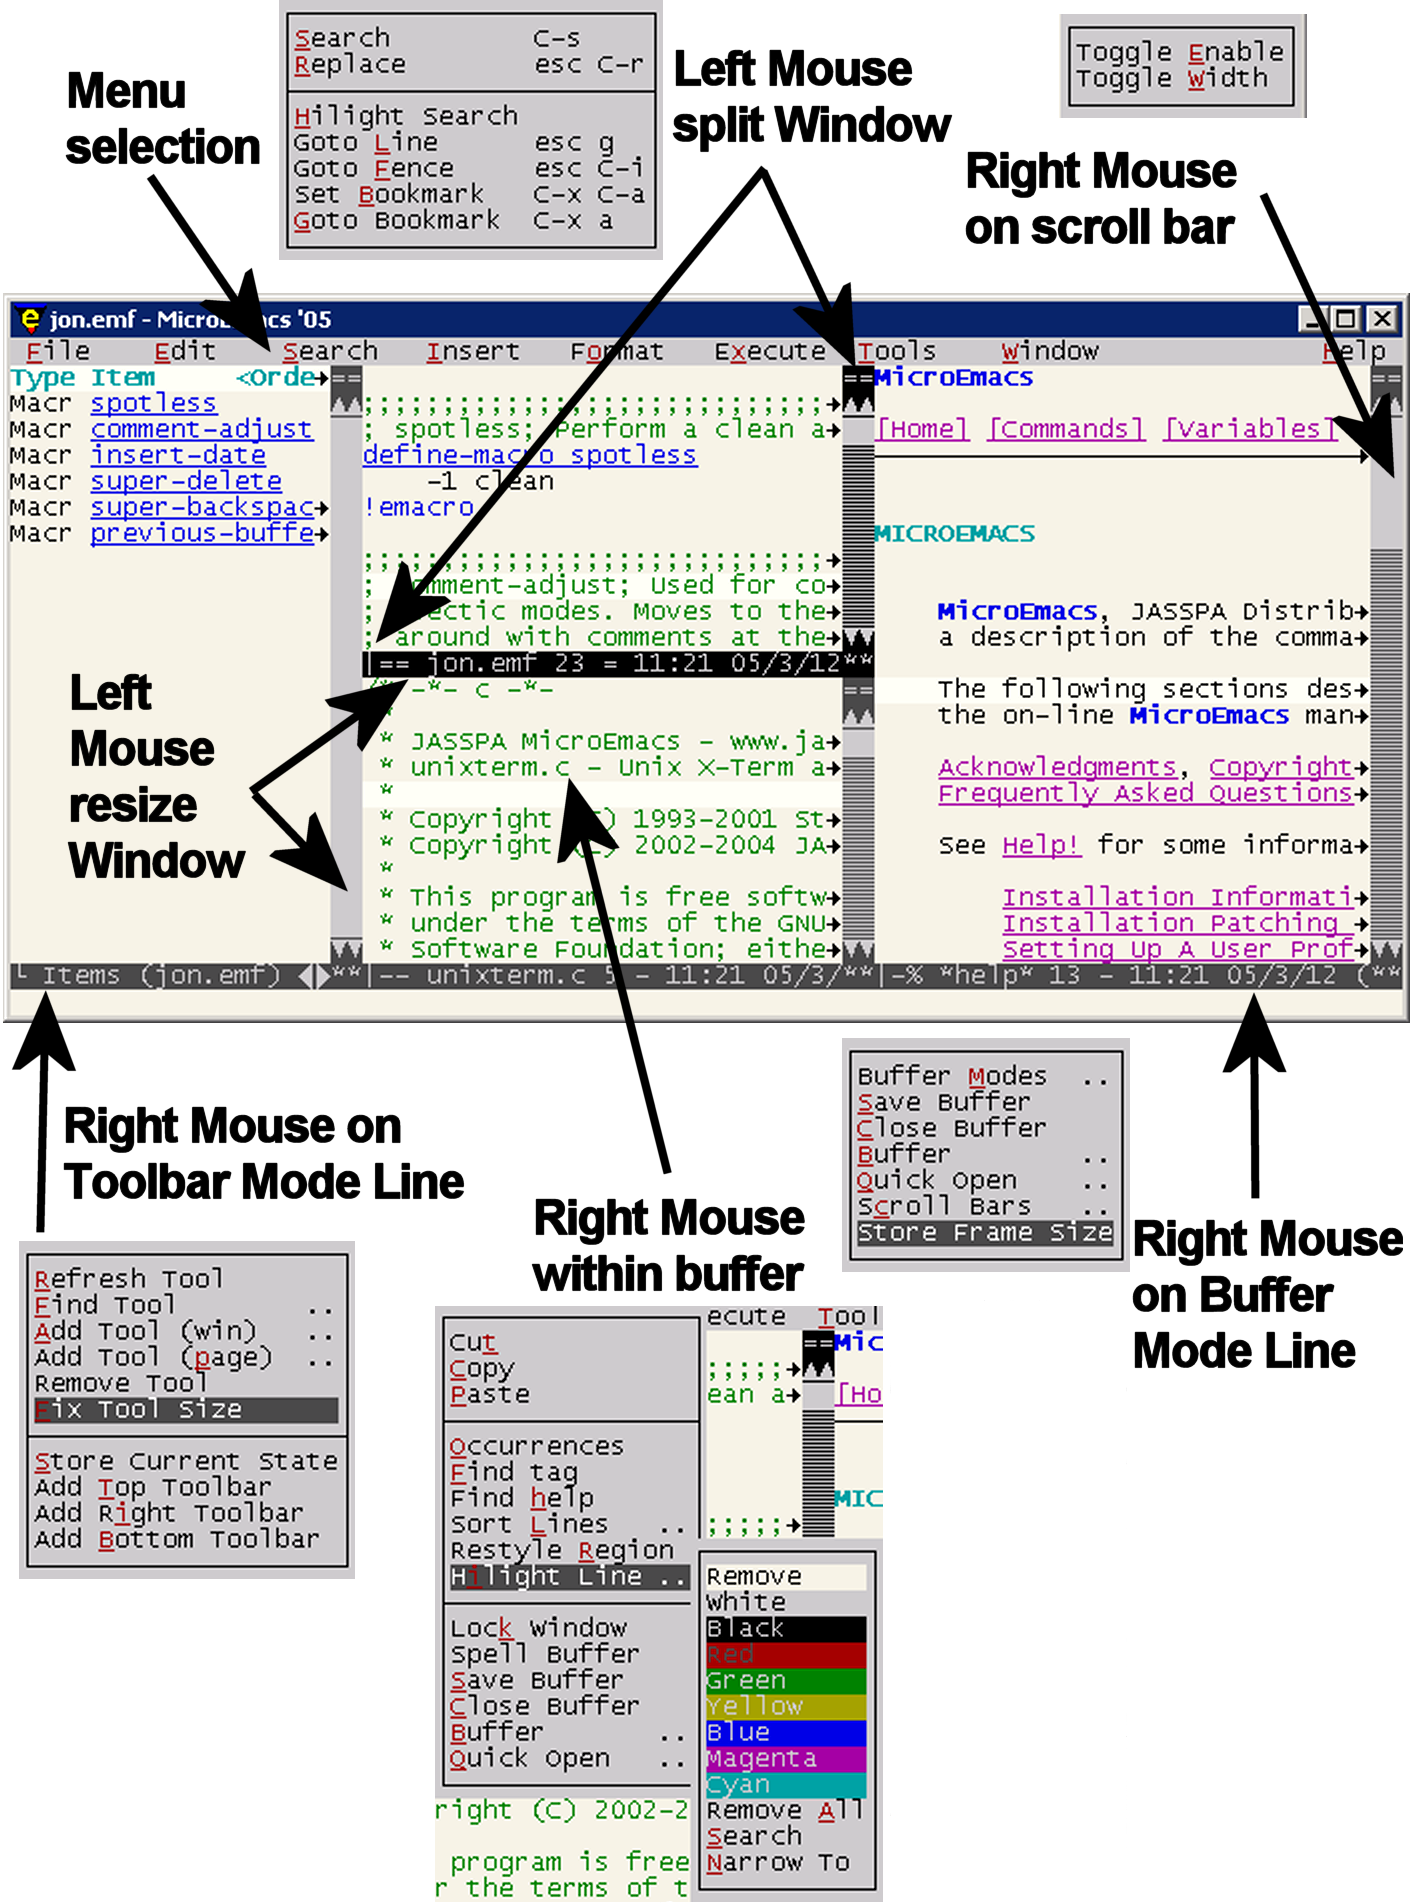
\includegraphics[keepaspectratio,width=.75\textwidth]{basicmouse}
      \caption{Basic mouse interaction}
      \label{fig:basicmouse}
    \end{center}
  \end{figure}

  The mouse interaction is configured from \textit{User Setup}

  \textbf{esc-x user-setup} $\dots$ \textit{OR}\newline
  \textbf{Help$\rightarrow$User Setup}

  using the \textbf{Mouse} tab. The tab defines the behavior of the mouse,
  including the mouse wheel. The default mouse interaction is summarized in
  Table~\ref{tab:mousecontrols}.

  \begin{center}
    \begin{small}
      \begin{longtable}{|p{.15\textwidth}|p{.2\textwidth}|p{.55\textwidth}|}
          \hline
          \textbf{Screen Region} & \textbf{Mouse Operation} &
          \textbf{Description}\\
          \hline
        \endhead
          \hline
          \caption {Mouse controls (continued $\ldots$)}
        \endfoot
          \hline
          \caption {Mouse controls}
          \label{tab:mousecontrols}
        \endlastfoot

        Buffer & Left Mouse\newline \textit{drag motion} &

        Selects a region of text. The text is automatically added to the
        \textit{yank buffer} and is available to external programs via the
        clipboard -- no explicit \textit{copy} operation is performed. \\
        \hline

        Buffer & Middle Mouse &

        Yanks the last selected region of text from the \textit{yank buffer}
        or \textit{clipboard} and inserts at the current mouse position. The
        behavior and button binding may be changed in \textit{User
        Setup::Mouse}.

        If the preferred behavior is for the text to be inserted at the cursor
        position rather than the mouse position then change the middle mouse
        button binding from \textbf{Move to Yank} to \textbf{No Move Yank}.\\
        \hline

        Buffer & Right Mouse &

        Pop-up context menu appears to interact with the buffer. The menu is
        context sensitive, if the right mouse is positioned over a spelling
        error when auto spell is enabled then alternative spelling corrections
        are displayed.

        The context menu may be invoked in a mouse-less system using
        \textbf{M-x context-menu} or via the short-cut key \textbf{S-F1}.\\
        \hline

        Scroll Bar & Right Mouse &

        Pop-up menu to change the width or enable state of the scroll bar. The
        default scroll bar attributes are set in \textit{User Setup}.\\ \hline

        Scroll Bar & Left Mouse\newline \textit{drag motion} &

        Vertical motion scrolls the buffer, horizontal motion resizes the
        width of the buffer window. If a window width is reduced to zero then
        the window is deleted.\\ \hline

        Scroll Bar & Left Mouse\newline \textit{splitter select} &

        If the window splitter option is enabled in \textit{User
        Setup::Platform::Scroll bars} then selecting the splitter at the top
        of the scroll bar causes the window to be split into two.\\ \hline

        Mode Line \newline \textit{Buffer} &
        Left Mouse\newline \textit{drag motion} &

        Vertical motion resizes the depth of the buffer window. If a buffer
        window depth is reduced to zero then the window is deleted.\\ \hline

        Mode Line \newline \textit{Buffer} & Right Mouse &

        Pop-up menu to control the buffer window appears. The menu allows the
        buffer to be closed, a new buffer to be opened in the window, etc.\\
        \hline

        Mode Line & Left Mouse\newline \textit{splitter select} &

        If the window splitter option is enabled in \textit{User
        Setup::Platform::Scroll bars} then selecting the splitter at the left
        of the mode bar causes the window to be split into two.\\ \hline

        Mode Line \newline \textit{Toolbar} & Right Mouse &

        Only valid when the \textbf{toolbar} is enabled (\textit{User
        Setup::Platform::Enable Toolbar}). A Pop-up menu appears to control
        the toolbar. The menu allows the toolbar content to be configured.\\

      \end{longtable}
    \end{small}
  \end{center}

\end{document}
